\begin{comment}
\documentclass[10pt]{article}
\usepackage{fullpage, graphicx, url}
\setlength{\parskip}{1ex}
\setlength{\parindent}{0ex}
\title{GEN07}
\begin{document}


\begin{tabular}{ccc}
The Alternative Csound Reference Manual & & \\
Previous & &Next

\end{tabular}

%\hline 
\end{comment}
\section{GEN07}
GEN07�--� Constructs functions from segments of straight lines. \subsection*{Description}


  Constructs functions from segments of straight lines. 
\subsection*{Syntax}


 \textbf{f}
 \# time size 7 a n1 b n2 c ...
\subsection*{Initialization}


 \emph{size }
 -- number of points in the table. Must be a power of 2 or power-of-2 plus 1 (see \emph{f statement}
). 


 \emph{a, b, c,}
 etc. -- ordinate values, in odd-numbered pfields p5, p7, p9, . . . 


 \emph{n1, n2}
, etc. -- length of segment (no. of storage locations), in even-numbered pfields. Cannot be negative, but a zero is meaningful for specifying discontinuous waveforms (e.g. in the example below). The sum \emph{n1}
 + \emph{n2}
 + .... will normally equal \emph{size}
 for fully specified functions. If the sum is smaller, the function locations not included will be set to zero; if the sum is greater, only the first \emph{size}
 locations will be stored. 


 


\begin{tabular}{cc}
\textbf{Note}
 \\
� &

 


 
\begin{itemize}
\item 

  If p4 is positive, functions are post-normalized (rescaled to a maximum absolute value of 1 after generation). A negative p4 will cause rescaling to be skipped. 

\item 

  Discrete-point linear interpolation implies an increase or decrease along a segment by equal differences between adjacent locations; exponential interpolation implies that the progression is by equal ratio. In both forms the interpolation from \emph{a}
 to \emph{b}
 is such as to assume that the value \emph{b}
 will be attained in the n + 1th location. For discontinuous functions, and for the segment encompassing the end location, this value will not actually be reached, although it may eventually appear as a result of final scaling. 


\end{itemize}


\end{tabular}

\subsection*{Examples}


  Here is a simple example of the GEN07 routine. It uses the files \emph{gen07.orc}
 and \emph{gen07.sco}
. It will create a single-cycle sawtooth whose discontinuity is mid-way in the stored function. Here is its diagram: 


 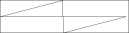
\includegraphics[scale=1]{gen07} 


 Diagram of the waveform generated by GEN07.


 \textbf{Example 1. A simple example of the GEN07 routine.}

\begin{lstlisting}
/* gen07.orc */
; Initialize the global variables.
sr = 44100
kr = 4410
ksmps = 10
nchnls = 1

; Instrument #1.
instr 1
  kamp = 30000
  kcps = 440
  ifn = 1

  ; Play the sine wave stored in Table #1.
  a1 oscil kamp, kcps, ifn
  out a1
endin
/* gen07.orc */
        
\end{lstlisting}
\begin{lstlisting}
/* gen07.sco */
; Table #1: a sawtooth wave (using GEN07).
f 1 0 256 7 0 128 1 0 -1 128 0

; Play Instrument #1 for 2 seconds.
i 1 0 2
e
/* gen07.sco */
        
\end{lstlisting}
\subsection*{See Also}


 \emph{GEN05}
, \emph{GEN06}
, and \emph{GEN08}

%\hline 


\begin{comment}
\begin{tabular}{lcr}
Previous &Home &Next \\
GEN06 &Up &GEN08

\end{tabular}


\end{document}
\end{comment}
